\section{Multijet QCD estimation} \label{sec:background:qcd}

The dominant background contribution to the SR comes from the non-resonant
multijet QCD process. Unfortunately the estimation of this process through MC
is not reliable due to the statistical precision of available samples and the
underlying inaccuracies of the event generation.  Thus, a data-driven estimate
was employed by fitting the large-$R$ jet mass distribution, $m_{J}$, in the SR
with a parametric function after validation of the procedure in the
$\text{CR}_{\text{QCD}}$.  This approach is further motivated by the good
agreement in shape of the $\text{CR}_{\text{QCD}}$ and SR over the mass range
of the fit, $70~\GeV$ to $230~\GeV$, as seen in
\Cref{fig:selection:sr_cr_shape}. A brief summary of this process is presented
below, with in-depth details available in Reference \cite{Feickert:2690521}.

It was found that the number of events in a $\sim 1~\ifb$ dataset from the
$\text{CR}_{\text{QCD}}$ is comparable to the number of events in the full
$80.5~\ifb$ SR dataset.  Thus, the $\text{CR}_{\text{QCD}}$ was broken into 60
slices constructed using adjacent data runs resulting in an average of
$1.2~\ifb$ of data per slice.

Two families of parametric functions were used for this modeling.  The
polynomial exponential function was chosen to be the nominal model

\begin{equation}
\label{sec:background:polynomial}
f_{n} \left(x \middle|\,\vec{\theta}\right) = \theta_{0}\, \exp\left(\sum_{i=1}^{n} \theta_{i}\,x^{i}\right), \quad x = \frac{m_{J} - 150~\GeV}{80~\GeV},
\end{equation}

and the alternative model, the formal Laurent series,

\begin{equation}
\label{sec:background:laurent}
f_{n} \left(x \middle|\,\vec{\theta}\right) = a \sum_{i=0}^{n} \frac{\theta_{i}}{x^{i+1}}, \quad a=10^{5},\,x = \frac{m_{J} + 90~\GeV}{160~\GeV}.
\end{equation}

The $\theta$ coefficients are determined by the fit, $a$ is empirically chosen
to keep the scale of parameters at $\mathcal{O}(1)$, and the independent
variable $x$ parameterizes the fit range $m_{J}\in[70,230]$ GeV to $x\in[-1,1]$
for \Cref{sec:background:polynomial} and $x\in[1,2]$ for
\Cref{sec:background:laurent}.  This reparameterization was empirically seen to
provide improved numerical stability in the fit.

Both functions are tested on a random $\text{CR}_{\text{QCD}}$ slice to
determine the minimum number of model parameters needed to describe the shape
of the distribution.  The $Z$ + jets, $W$ + jets, and $k$-factor corrected
$t\bar{t}$ contributions are all scaled by their cross sections times the
luminosity and then subtracted from the slice to remove bias from the fit.  The
results of a likelihood ratio test with Wilks' theorem \cite{wilks1938} and the
$F$-test \cite{snecdecor1991statistical} were both used to determine the
minimum number of model parameters for both function choices.  The two
statistical tests were performed for all $\text{CR}_{\text{QCD}}$ data slices
and the relative frequencies of the observed $p$-values were iteratively summed
as shown in \Cref{sec:background:parameter_tests} for both function choices.
The Wilks test preferred a five-parameter model for both while the $F$-test
preferred a four-parameter model for both.  To be conservative in the final
estimate, the five-parameter model was chosen for both the polynomial
exponential function and the formal Laurent series.

\begin{figure}[!htbp]
\centering
\subcaptionbox{Polynomial exponential Wilks test\label{sec:backgrounds:poly_wilks_test}}{
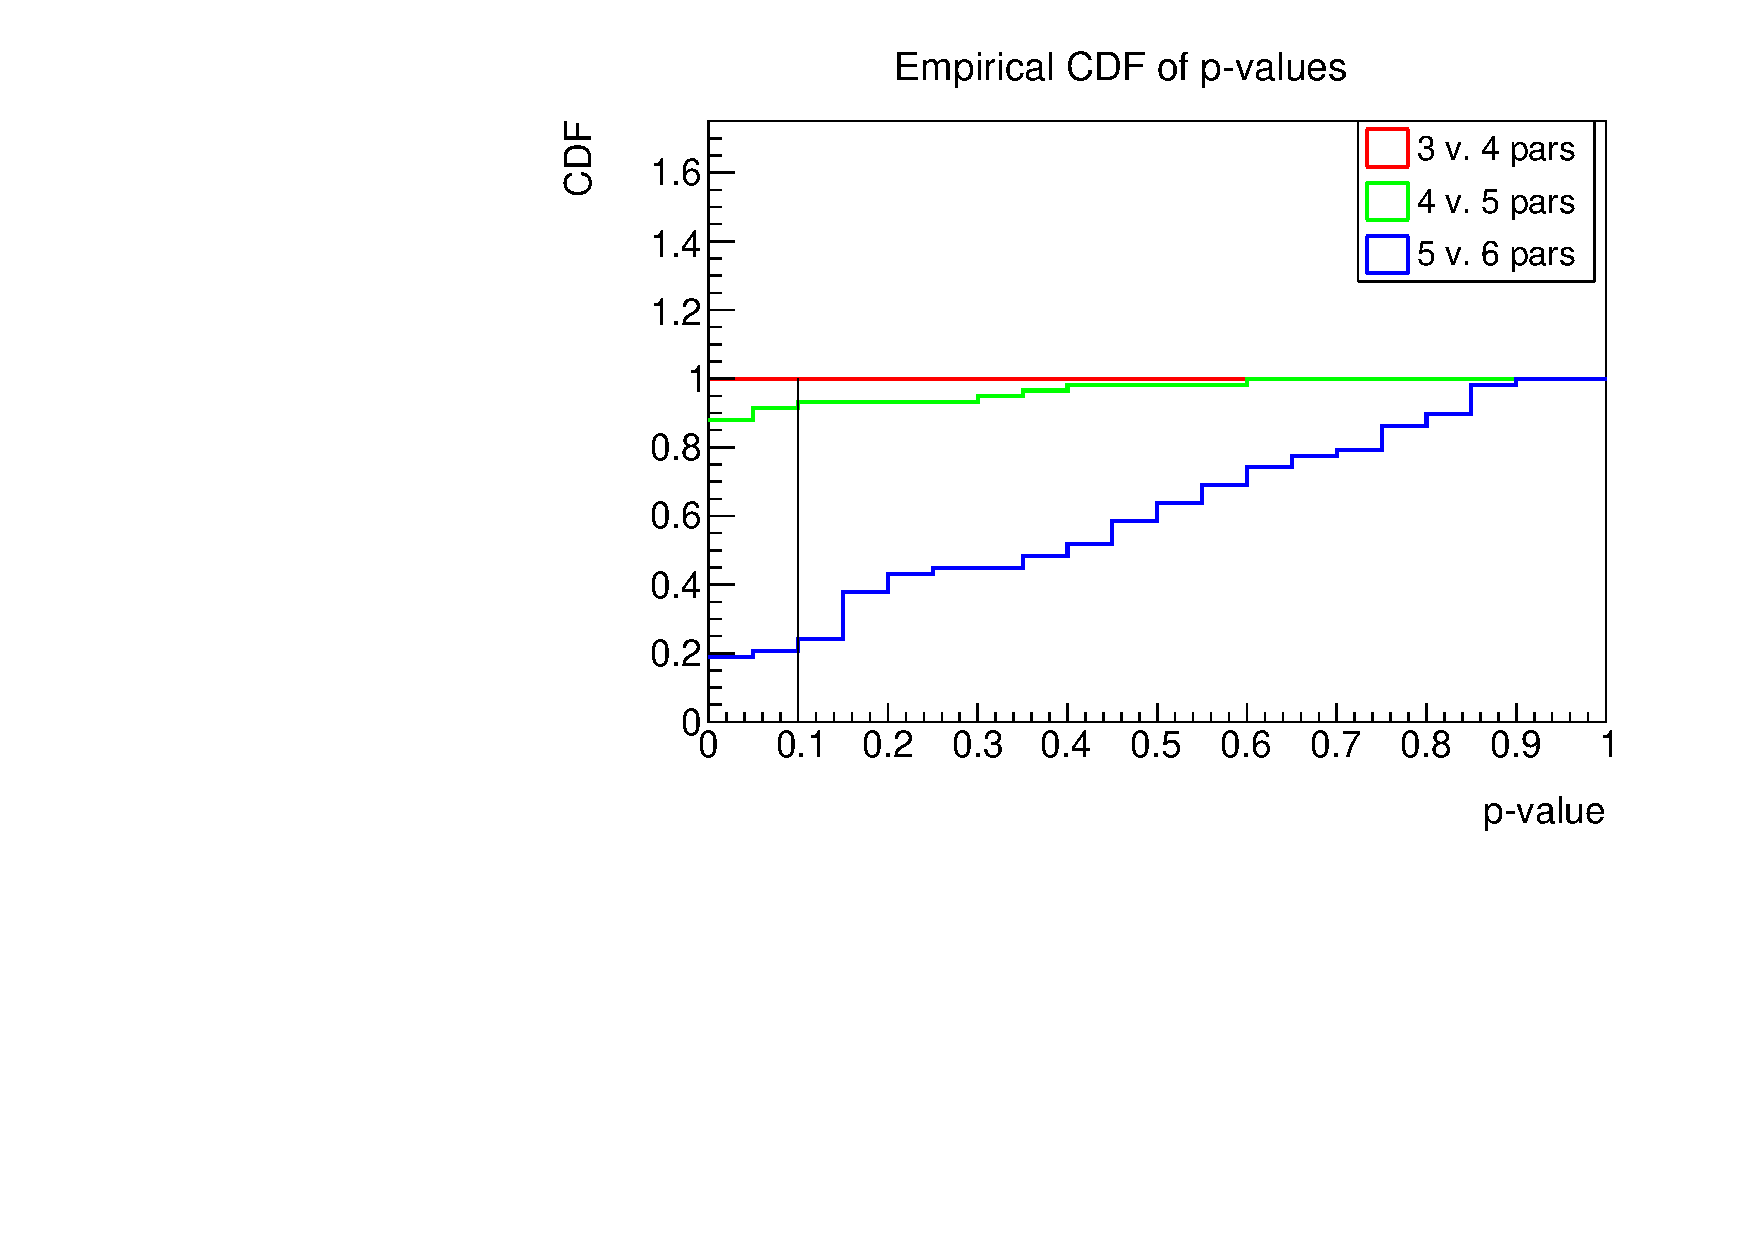
\includegraphics[width=0.48\linewidth]{figures/backgrounds/poly_wilks_test}
}\hfill
\subcaptionbox{Polynomial exponential F test \label{sec:backgrounds:poly_f_test}}{
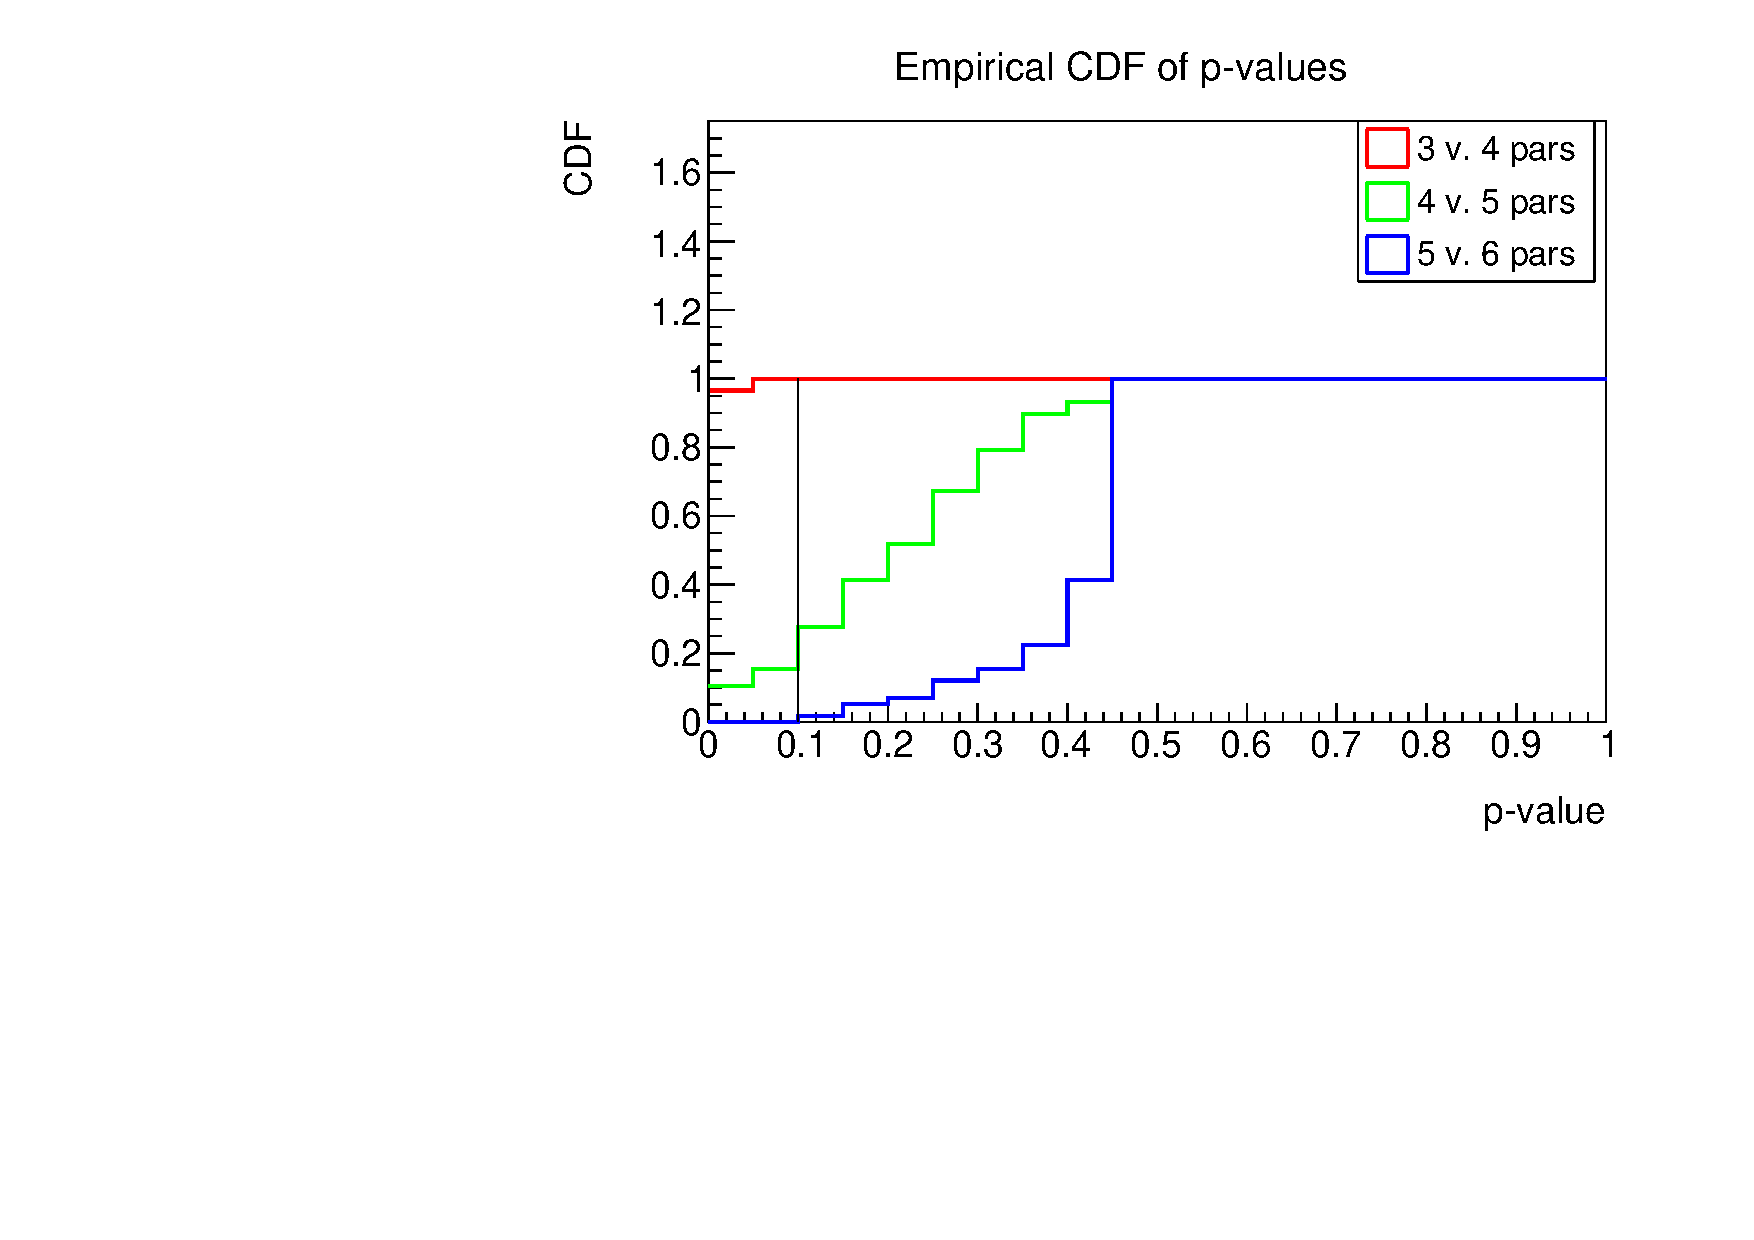
\includegraphics[width=0.48\linewidth]{figures/backgrounds/poly_f_test}
}
\subcaptionbox{Formal Laurent Wilks test\label{sec:backgrounds:formal_wilks_test}}{
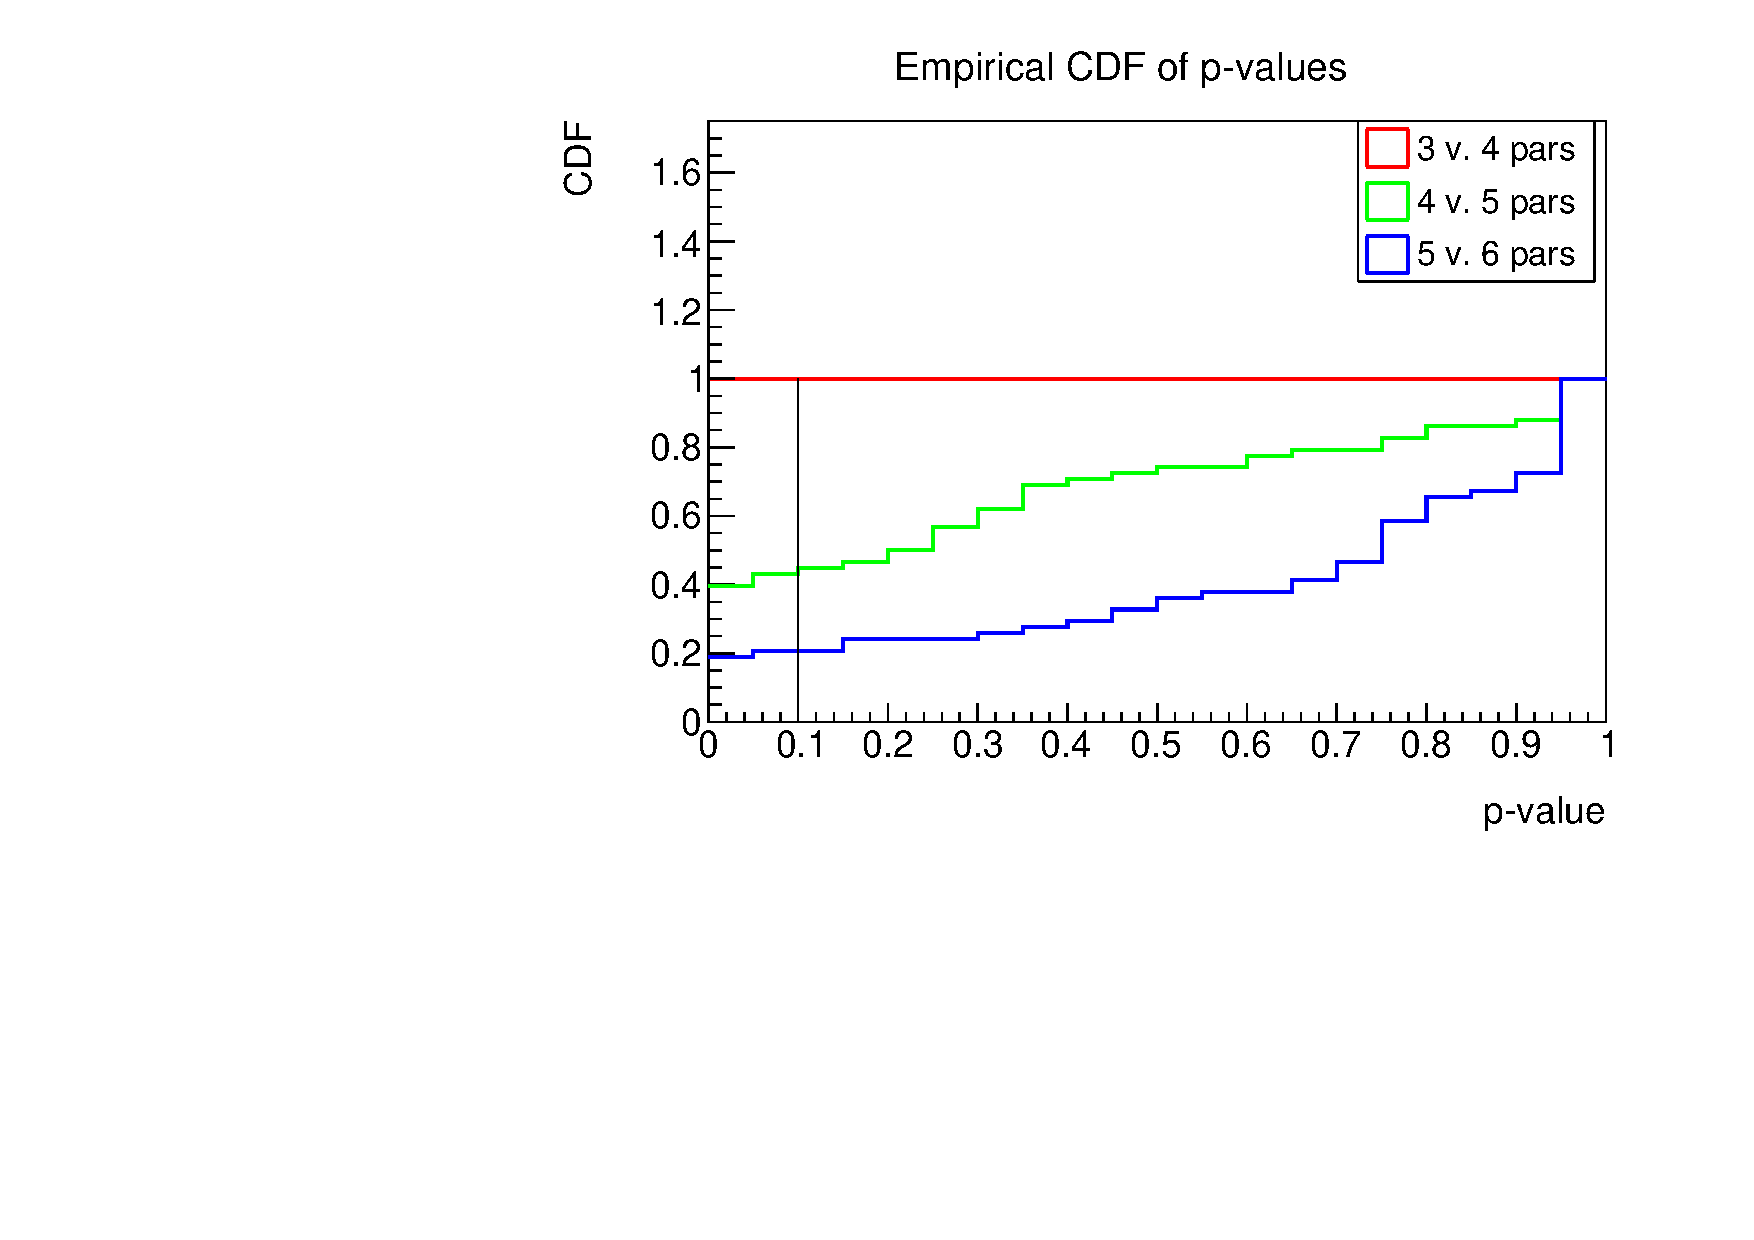
\includegraphics[width=0.48\linewidth]{figures/backgrounds/formal_wilks_test}
}\hfill
\subcaptionbox{Formal Laurent F test \label{sec:backgrounds:formal_f_test}}{
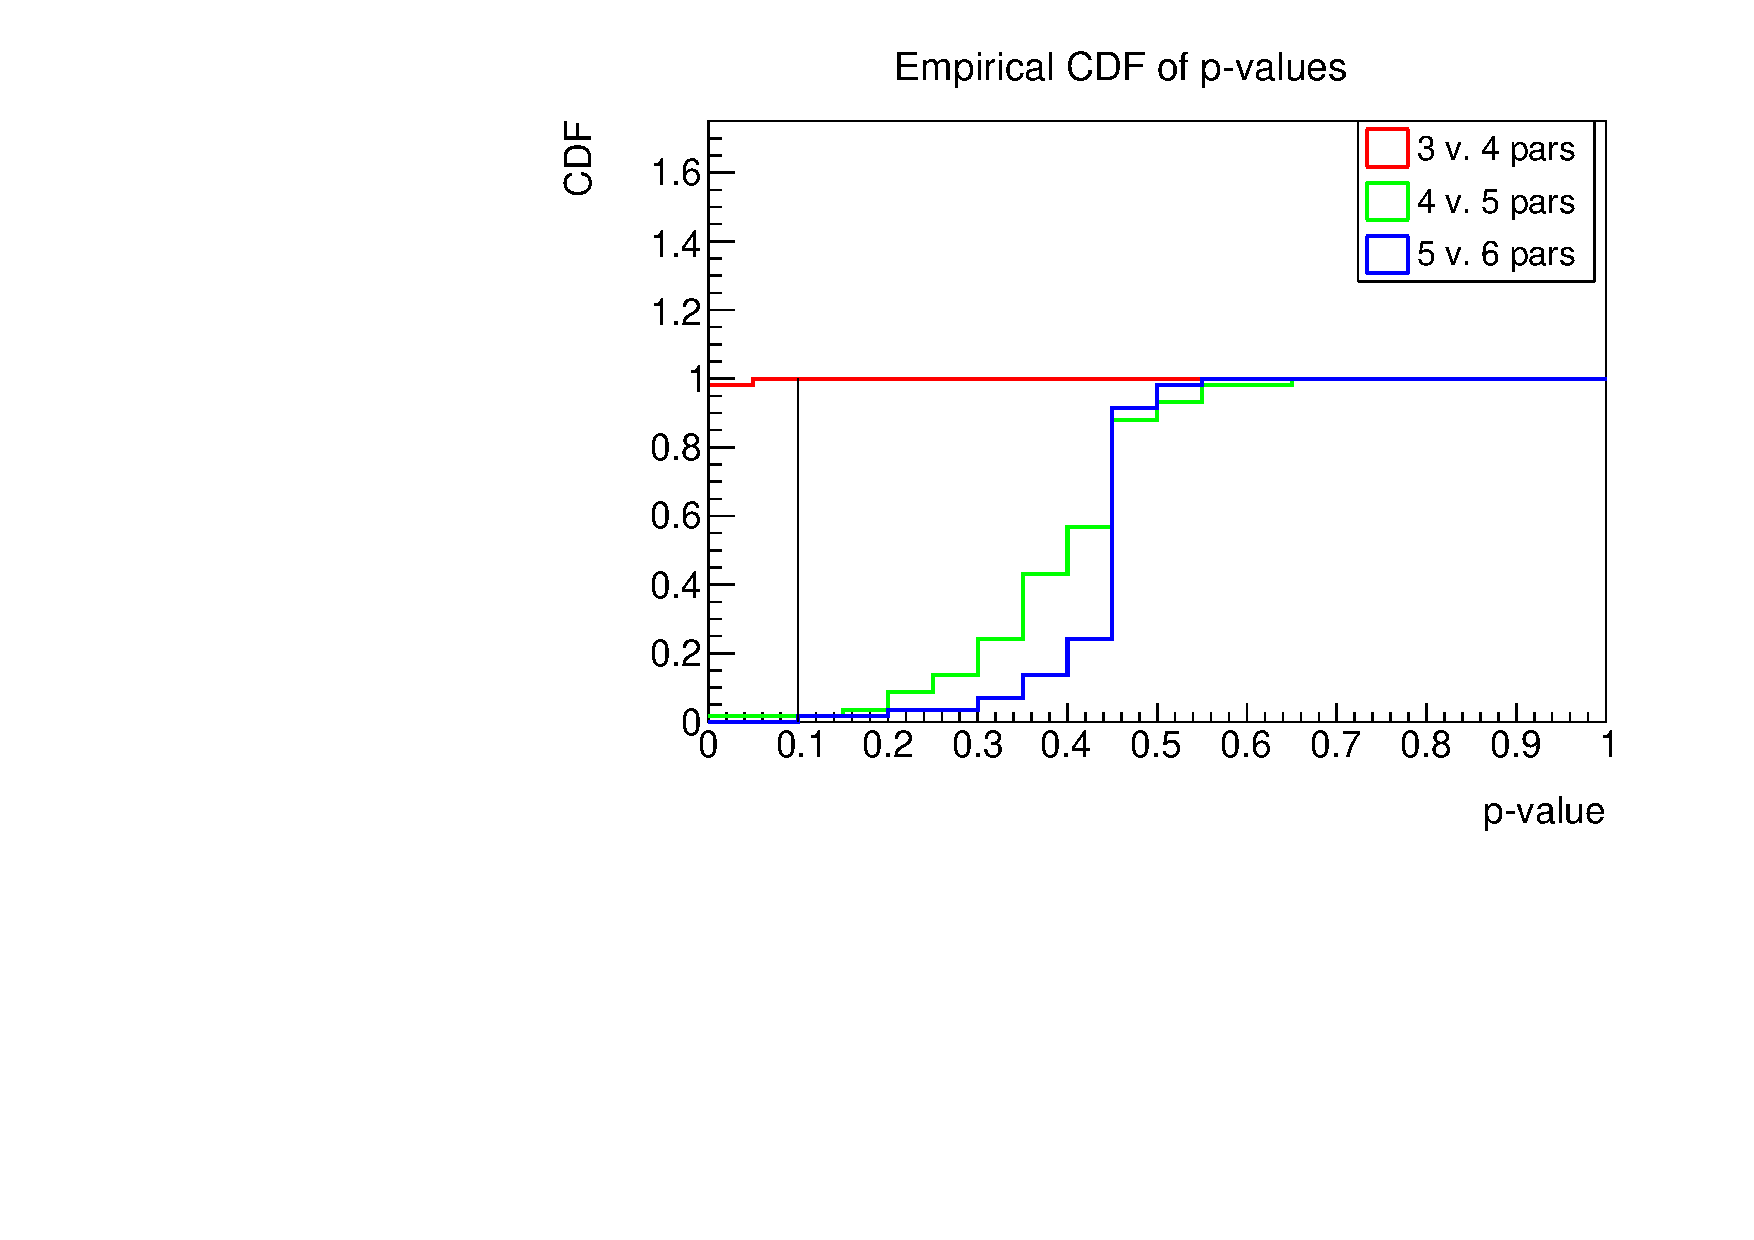
\includegraphics[width=0.48\linewidth]{figures/backgrounds/formal_f_test}
}
\caption{Empirical cumulative distribution function (CDF) for the test
$p$-values for the two statistical tests applied to both function choices where
the a priori threshold $\alpha$ is shown as a vertical black line. In both
tests $p$-values below $\alpha = 0.1$ show preference for the model with more
parameters, while $p$-values above $\alpha = 0.1$ indicate a preference for the
model with fewer parameters \cite{Alison:2649017}.}
\label{sec:background:parameter_tests}
\end{figure}

In order to determine the robustness of these fit functions, they were validated
using all of the $\text{CR}_{\text{QCD}}$ slices.  For these validation studies
the fit included properly scaled $Z$ + jets, $W$ + jets, $t\bar{t}$ and single
top contributions in addition to the $\text{CR}_{\text{QCD}}$ slice. Within the
statistical precision given by the different data slices, the $\chi^{2}/\text{ndf}$
from the individual fits is found to follow the expected distribution of a good
fit.
